\chapter{DESIGN AND IMPLEMENTATION}
\label{chap:desainandimplementation}

% Ubah bagian-bagian berikut dengan isi dari desain dan implementasi

Penelitian ini dilaksanakan sesuai \lipsum[1][1-5]

\section{Make New Dataset}
\label{sec:makenewdataset}

This new dataset is a merge of KimbRo's Humanoid Robot Pose dataset and Ichiro's dataset. NimbRo's dataset contains both single and multiple robots to
simulate RoboCup's real conditions. They also gathered from RoboCup Humanoid League YouTube videos, their own internal videos, and ROS bags. 
Overall, their dataset has over 1.5k images that come from 23 videos with around 2.3k robot instances. These images include teen and adult-sized robots and contain more than ten different robot types \parencite{amini2021}.
However, the robots in Ichiro's dataset are only kid-sized and come in single or maximum two-robot configurations. The images in our dataset come from videos that are taken in our lab. 
Then we split up those videos into multiple images and we pick not blurred videos.
Before merging, we need to fix NimbRo's dataset format first. This is because after we visualized some of their data, we found that the bounding boxes in \emph{annotations} part were misplaced (the width and height were swapped).
After we refine their dataset format and merge them with our dataset, the newly created dataset has approximately 2.5k images.
About 20 percent of the dataset was used for scoring and validating.

When it comes to annotation tools, there are a lot of choices out there including offline and online tools. We have tried some of them like Dataloop, V7labs, or Supervisely which is recommended by NimbRo.
However, when we tried to export the dataset into COCO format, it failed (e.g. can not import it or it can be imported but the JSON result in the annotation section is none). So, we decided to use a coco-annotator,
a web-based image annotation tool designed for versatility and efficiently labeling images to create training data. Regarding the number of keypoints in each robot, we followed NimbRo's dataset.
There are six keypoints including head, trunk, hands, and feet. We stick to that idea because we want to try the model's performance and inference time with fewer keypoints first and if we are confident enough, we will increase the number of keypoints later.

\section{Training Pose Estimation Model for Humanoid Robot}
\label{sec:trainingrobot}

All of the training processes in this study were primarily conducted on a DGX-A100 server computer and written in the Python programing language. The specific configuration explains in Table \ref{tb:dgxa100}.
From this base specification, we are allocated a Jupiter notebook container with
python and many libraries preinstalled with following allocated resources explained in Table \ref{tb:allocatedcontainer}.

\begin{longtable}{|c|c|}
  \caption{DGX-A100 Specification.}
  \label{tb:dgxa100}\\
  \hline
  CPU     & Dual AMD Rome 7742, 128 cores total @ 2.25 GHz \\
  \hline
  GPU     & 8 x NVIDIA A100 80 GB Tensor Core GPUs  \\
  \hline
  RAM     & 2 TB \\
  \hline
  Storage & 30 TB (8 x 3.84 TB) U.2 NVMe drives \\
  \hline
\end{longtable}

\begin{longtable}{|c|c|}
  \caption{Allocated container specification.}
  \label{tb:allocatedcontainer}\\
  \hline
  GPU     & 1/4 NVIDIA A100 GPU \\
  \hline
  GPU RAM & 20 GB  \\
  \hline
  CPU RAM & 8 GB \\
  \hline
  Storage & 100 GB  \\
  \hline
\end{longtable}

\subsection{NimbRo's Model}
\label{subsec:nimbro-model}

There are three Pose Estimation Models for humanoid robots that we retrained with the new dataset. All of them used bottom-up approaches. The first one is NimbRo's model,
they chose to use a similar architecture with NimbRo-Net and NimbRo-Net2 because it had such positive outcomes. Their model is an single-stage encoder-decoder network which takes an RGB image of
size \emph{w x h}. The model predicts heatmaps of both keypoints and limbs for scale 1/4 and only
heatmaps of keypoints for scale 1/2, where each scale is supervised with an intermediate loss \parencite{amini2021}. The full network architecture is depicted in Figure \ref{fig:nimbro-model-architecture}.

\begin{figure}[ht]
  \centering
  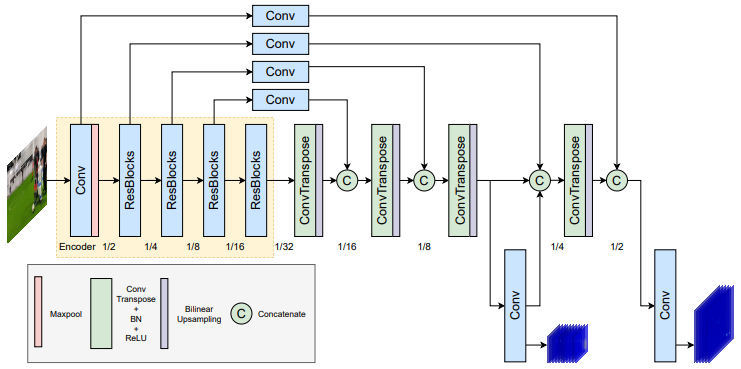
\includegraphics[scale=0.9]{gambar/nimbro-architecture.png}
  \caption{NimbRo's model architecture}
  \label{fig:nimbro-model-architecture}
\end{figure}

The hyperparameters that are used to train NimbRo's model followed the description in their paper.
This model is trained using the AdamW optimizer with a learning rate of 10\textsuperscript{-4} ,
batch size 16, and weight decay of 10\textsuperscript{-4} for the total 200 epochs.
Note that the encoder is initialized by pre-trained ResNet weights on ImageNet.
We also use data augmentation that includes random horizontal flip, random
rotation, random scaling, and random translation during training \parencite{amini2021}.

\subsection{YOLO-pose}
\label{subsec:YOLO-pose}

Another model that we trained with new dataset is YOLO-pose. Although this architecture is intended for humans, but it may be used for humanoid robot too, as explained in Section \ref{subsec:humanoidrobotposeestimation}.
YOLO-pose is a single-shot approach like other bottom-up approaches. However, it doesn't use heatmaps. Rather, it associates all keypoints of a person with anchors. It is
based on YOLOv5 object detection framework and can be extended to other frameworks as well. Figure \ref{fig:YOLO-pose-architecture} illustrates the overall architecture with keypoint
heads for pose estimation. The Input image is passed through darknetcsp backbone that generates feature maps at
various scales {P3, P4, P5, P6}. PAnet is used for fusing these feature maps across multiple scales and the output is fed to detection
heads. Finally each detection head branches into box head and keypoint head \parencite{maji2022yolopose}.

\begin{figure}[ht]
  \centering
  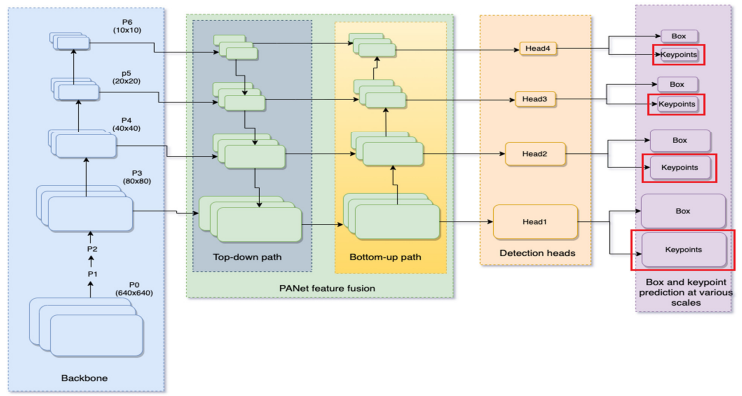
\includegraphics[scale=1]{gambar/yolo-architecture.png}
  \caption{YOLO-pose architecture.}
  \label{fig:YOLO-pose-architecture}
\end{figure}

Before we jumped into training process, we must change format of our newly dataset from COCO to YOLO. Differ from COCO format, YOLO format give keypoint confidence or visibility flag 2 for either visible or occluded keypoint
and if it is outside the field of view, the value is set to zero. However, COCO format defined visibility flag as v=0: not labeled,  v=1: labeled but not visible, and v=2: labeled and visible. So, we change the definition of
v=1 and v=2 become just v=2 in YOLO format and keep v=0.
Beside keypoint format differences, bounding-box format between them is also different. COCO defines a bounding-box as follow: x (top left), y (top left), width, and height. On the other hand,
bounding-box format in YOLO is: x (center), y (center), width, and height also all of them need to be normalized. Thus, we need to add 1/2 width to x, 1/2 height to y, and normalize them.
All of that processes can be seen in Code \ref{lst:changecocotoyolo}. 

\lstinputlisting[
  language=Python,
  caption={Change COCO to YOLO format program.},
  label={lst:changecocotoyolo}
]{program/coco-to-yolo.py}

The hyperparameters to train YOLO-pose followed the description in their GitHub named \emph{hyp.pose.yaml}.
We use SGD optimizer with a cosine scheduler. The base learning rate is set to 10\textsuperscript{-2}, batch size 16,
and weight decay of 5\textsuperscript{-4} for total 150 epochs. There are also data augmentation like random scale ([0.5, 1.5]),
random translation [-10, 10], random flip with probability 0.5, mosaic augmentation with probability 1, and various color augmentations.

\section{Implementasi Alat
  \label{sec:implementasi alat}}

Alat diimplementasikan dengan \lipsum[1]

% Contoh pembuatan potongan kode
\begin{lstlisting}[
  language=C++,
  caption={Program halo dunia.},
  label={lst:halodunia}
]
#include <iostream>

int main() {
    std::cout << "Halo Dunia!";
    return 0;
}
\end{lstlisting}

\lipsum[2-3]

% Contoh input potongan kode dari file
\lstinputlisting[
  language=Python,
  caption={Program perhitungan bilangan prima.},
  label={lst:bilanganprima}
]{program/bilangan-prima.py}

\lipsum[4]
